\section{Introduction}
Navigation is one of the fundamental tasks in mobile robotics. For robots with reasonable dynamics and operating speeds in indoor environments, efficient collision-free navigation is practically solved. However, introducing constraints other than ``please take the shortest path without running into anything'' is an ongoing area of research, especially for taking the social needs of humans into account. However, the best methods and parameters for adding the constraints has not been adequately explored. 

\begin{figure}
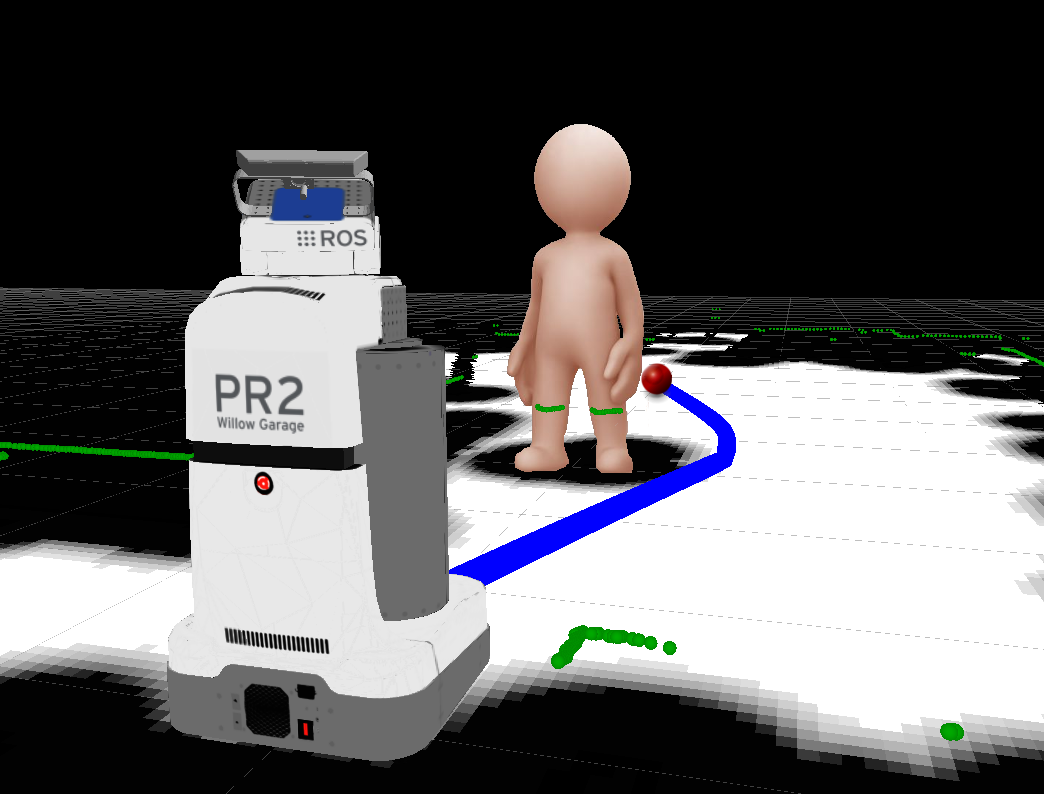
\includegraphics[width=\columnwidth]{graphix/pr2base.png}\\
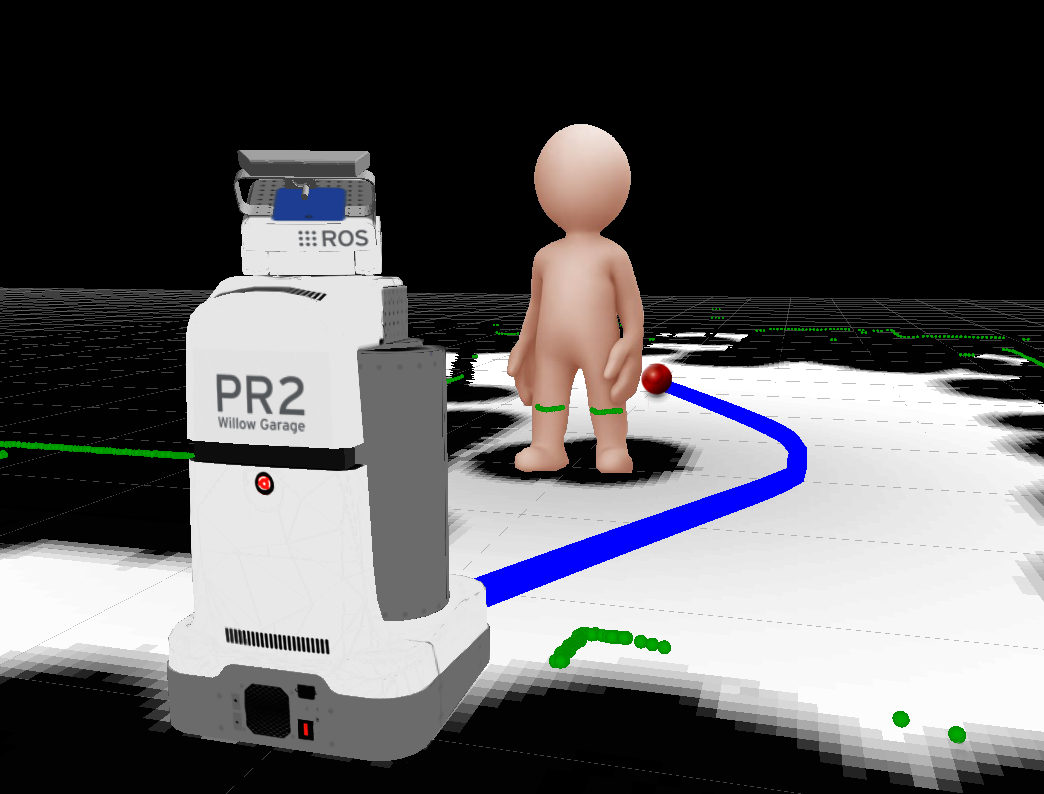
\includegraphics[width=\columnwidth]{graphix/pr2social.png}
\caption{Respecting Personal Space with a Soft Constraint - The top picture shows a typical collision-free path that comes too close for comfort to the person. By adding a Gaussian distribution to the costmap around the person, the planned path gives the person more space.}
\label{fig:intro}
\end{figure}

Consider the path in the top part of Figure \ref{fig:intro}. The robot planned the shortest path that does not collide with any objects. However, that does not make it the optimal path. This path drives almost straight at the person, comes within centimeters of them and enters their personal space. The path is legal and valid, but it treats the person like any other obstacle. The robot drives around the person like it would any other object or piece of furniture. The path planned in the bottom part of Figure \ref{fig:intro} is much better since it affords the person more of their personal space. 

Both scenarios can be achieved by path planning on a costmap. However, the planner that generated the path on the top treats the costmap as an Occupancy Grid\cite{matthies1988}, where the world is discretized into cells, each labeled occupied or free. The occupied cells are considered ``lethal'' since they would result in a collision for the robot. A more general costmap, like the one used by the planner in the bottom picture can have a whole range of values (represented by $f(x,y)$). The lethal cells are greater than some limit $L$, the free cells are marked with $f(x,y)=0$ and everything in between is a ``non-lethal'' obstacle. 

What does it mean for a cell to be non-lethal? They can mark places where there might be an obstacle, but more interestingly they can denote locations where it is undesirable to be for one reason or another and does \emph{not} result in a collision. Raising the value of the cells makes it less likely for the robot to travel into those cells. But how much less likely? Under what conditions? The answer is, it depends. 

The intermediate non-lethal cells are the key to representing the soft constraints. They are useful for representing general preferences/guidelines rather than hard and fast rules. Policies such as ``do not enter the kitchen unless there is no other path'' and ``leave some room between you and the wall when you can'' can easily be implemented as soft constraints. The most frequently used scenario for such obstacles, though, is for representing a person's preferences for how to interact with a robot. As \citet{kirby:companion} observed, ``Human social conventions are tendencies, rather than strict rules,'' arguing that the binary costmap (occupied/unoccupied) is inadequate for representing human constraints. The benefit of soft constraints is that the path through non-lethal obstacles on the costmap are still valid, just less preferable. The robot can still enter a person's personal space, or enter the kitchen, if there are no better options. Creating paths from non-lethal costmaps gives roboticists a way to rank multiple different legal options for some metric based on the desired behavior. 

The choice of which path is taken and which path is less traveled depends on two separate components. The first is the costmap itself, which can be statically generated or created from sensor data. Second, the path planning algorithm itself calculates the path with the least total cost. The standard algorithms such as Dijikstra's and A* can be used. To optimize for path length (and thus avoid wayward paths that avoid every hint of an obstacle), wavefront planners are often used, which add a constant value to each cell traversed to create a gradient from start to finish\cite{choset:principles}. The interplay between the values in the costmap and the path planning constant turns out to be crucial for determining which path is optimal. 

Creating the desired behavior is more difficult than one would expect. While previous researchers have tuned their parameters to create working configurations, there exists no general guide for how to tune the parameters to change the robot behavior. Furthermore, as our exploration of this space shows, the behavior is not always readily intuitive. 

%This paper aims to explore the space of these paths through non-lethal costmaps. 

%Occupancy Grids have proven useful over the years because their volumetric representation allows for unstructured data from heterogeneous sources. These binary values are used to construct a graph with which planning can be done using Dijkstra's algorithm or any of its variants. However, such Occupancy Grids cannot represent non-lethal obstacles. The more advanced representation of costmaps can take any arbitrary number of values, however, in practice, such grids often devolve into the highest values representing occupied, the lowest representing unoccupied, and everything in between is largely untouched. 


